\let\negmedspace\undefined
\let\negthickspace\undefined
\documentclass[journal]{IEEEtran}
\usepackage[a5paper, margin=10mm, onecolumn]{geometry}
%\usepackage{lmodern} % Ensure lmodern is loaded for pdflatex
\usepackage{tfrupee} % Include tfrupee package

\setlength{\headheight}{1cm} % Set the height of the header box
\setlength{\headsep}{0mm}     % Set the distance between the header box and the top of the text

\usepackage{gvv-book}
\usepackage{gvv}
\usepackage{cite}
\usepackage{amsmath,amssymb,amsfonts,amsthm}
\usepackage{algorithmic}
\usepackage{graphicx}
\usepackage{textcomp}
\usepackage{xcolor}
\usepackage{txfonts}
\usepackage{listings}
\usepackage{enumitem}
\usepackage{mathtools}
\usepackage{gensymb}
\usepackage{comment}
\usepackage[breaklinks=true]{hyperref}
\usepackage{tkz-euclide} 
\usepackage{listings}
% \usepackage{gvv}                                        
\def\inputGnumericTable{}                                 
\usepackage[latin1]{inputenc}                                
\usepackage{color}                                            
\usepackage{array}                                            
\usepackage{longtable}                                       
\usepackage{calc}                                             
\usepackage{multirow}                                         
\usepackage{hhline}                                           
\usepackage{ifthen}                                           
\usepackage{lscape}
\usepackage{multicol}
\begin{document}

\bibliographystyle{IEEEtran}
\vspace{3cm}

\title{4.13.17}
\author{EE25BTECH11012-BEERAM MADHURI}
% \maketitle
% \newpage
% \bigskip
{\let\newpage\relax\maketitle}

\renewcommand{\thefigure}{\theenumi}
\renewcommand{\thetable}{\theenumi}
\setlength{\intextsep}{10pt} % Space between text and floats


\numberwithin{equation}{enumi}
\numberwithin{figure}{enumi}
\renewcommand{\thetable}{\theenumi}


\textbf{Question}:\\
Three distinct points $A$, $B$ and $C$ are given in the 2-dimensional coordinate plane such that the ratio of the distance of any one of them from the point $(1,0)$ to the distance from the point $(-1,0)$ is equal to $\frac{1}{3}$. Then the circumcentre of the triangle $ABC$ is at the point:
\begin{enumerate}
\begin{multicols}{4}
\item $\left(\frac{5}{4}, 0\right)$
\item $\left(\frac{5}{2}, 0\right)$
\item $\left(\frac{5}{3}, 0\right)$
\item $(0, 0)$
\end{multicols}
\end{enumerate}
\textbf{Solution:}
let $\vec{F_1}$, $\vec{F_2}$ be the vectors such that:
\begin{table}[h!]
    \centering
    \begin{tabular}[12pt]{ |c| c|}
    \hline
    \textbf{Point} & \textbf{Vector}\\ 
    \hline
    $\myvec{F_1}$ &  $\myvec{1\\0}$\\
    \hline
    $\myvec{F_2}$ &   $\myvec{-1\\0}$\\
    \hline
    \end{tabular}
    \caption{Variables used}
    \label{table 1.9.1}
\end{table}\\
  Let P $\myvec{x\\y}$ be any point in the plane of A,B,C.\\
  given,
\begin{align}
\frac{\| PF_1 \|}{\| PF_2 \|} = \frac{1}{3}\\
\frac{\sqrt{(P-F_1)^T (P-F_1)}}{\sqrt{(P-F_2)^T (P-F_2)}} = \frac{1}{3}
\end{align}
By Substituting Values and Simplifying:
\begin{align}
2x^2 + 2y^2 - 5x + 2 = 0\\
\left\lVert
\begin{pmatrix} x \\ y \end{pmatrix}
-
\begin{pmatrix} \tfrac{5}{4} \\ 0 \end{pmatrix}
\right\lVert
= \sqrt{\tfrac{21}{4}}
\end{align}
On comparing the equation with general form:-
\begin{align}
||P - C|| = r\\
\text{
where ,}
\text{
P = any point on the circle}\\
\text{C = Center of circle}\\
\text{
r = radius of circle}\\
\text{
Center of circle =  } (\frac{5}{4}, 0)
\end{align}
Hence, the circumcenter of the triangle is $(\frac{5}{4}, 0)$
\begin{figure}[H]
    \centering
    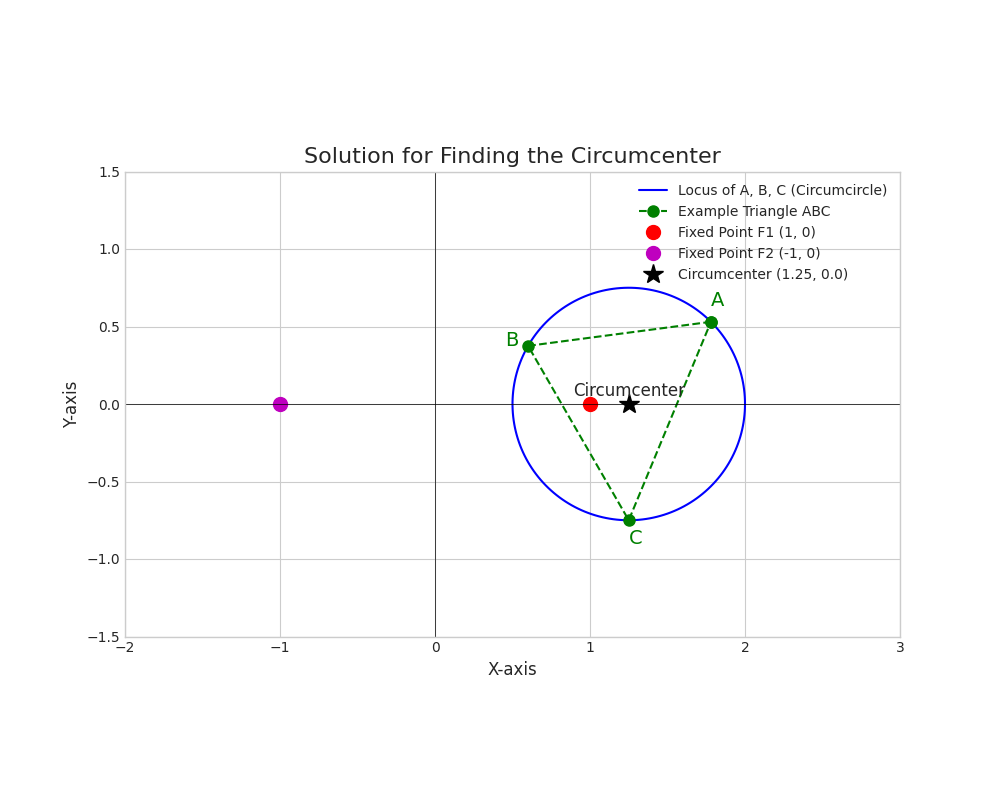
\includegraphics[width=0.85\columnwidth]{figs/graph9.png}
    \caption{4.13.17}
    \label{fig:placeholder}
\end{figure}

\end{document}